\documentclass{ximera}
\usepackage{listings}
\usepackage{tikz}
\usetikzlibrary{shapes.geometric, arrows}

\tikzstyle{startstop} = [rectangle, rounded corners, minimum width=3cm, minimum height=1cm, text centered, fill=red!50]
\tikzstyle{io} = [trapezium, trapezium left angle=70, trapezium right angle=110, minimum height=1cm, text centered, fill=blue!30]
\tikzstyle{process} = [rectangle, minimum width=3cm, minimum height=1cm, text centered, text width=3cm, fill=orange!50]
\tikzstyle{decision} = [diamond, minimum width=3cm, minimum height=1cm, text centered, text width=2cm, fill=green!30]
\tikzstyle{arrow} = [thick,->,>=stealth]

\title{If/Else Statements}
\begin{document}
\lstset{language=Python,frame=tb}
\begin{abstract}
We introduce if/else statements in Python.
\end{abstract}
\maketitle

\section{If/Else}

In an earlier section we saw that in order to compute the absolute value of a real number $x$, we first needed to determine if it satisfied a certain condition, namely, is it the case that $x>0$? The answer to this question then determines the set of instructions to follow. We can reformulate our algorithm for computing $|x|$ as two statements in the following ways:

For any real number $x$, if $x>0$, then $|x|=x$. Else (or otherwise), $|x|=-x$.

The `if' portion of the statement explains what to do if the given condition is satisfied, while the `else' portion explains what to do if the given condition is not satisfied.

We can express the same idea as above in pseudocode below. (Note that pseudocode will look a lot like Python syntax, but they are not the same.)

\begin{verbatim}
===PSEUDOCODE=================
procedure absolute(x: real number)
        IF x > 0, THEN absVal = x
        ELSE absVal = -x
        RETURN absVal (the absoluve value of x)
==============================
\end{verbatim}

The block of pseudocode above has several important features:

\begin{itemize}
	\item The word \verb|absolute| is the name of this algorithm.
	\item The \verb|x| in parentheses is the input.
	\item The \verb|IF|, \verb|THEN|, \verb|ELSE|, etc. represent keywords in the individual steps taken in the algorithm. (For a more complete treatment of this, see Rosen's Discrete Mathematics and Its Applications textbook.)
	\item The term \verb|absVal| is a variable used to compute the absolute value of \verb|x|.
	\item The variable after the \verb|RETURN| keyword is what the procedure outputs.
\end{itemize}

These two new ways of expressing an algorithm can be easily mapped to the flowchart for computing $|x|$ below (see Figure 1).

\begin{center}
    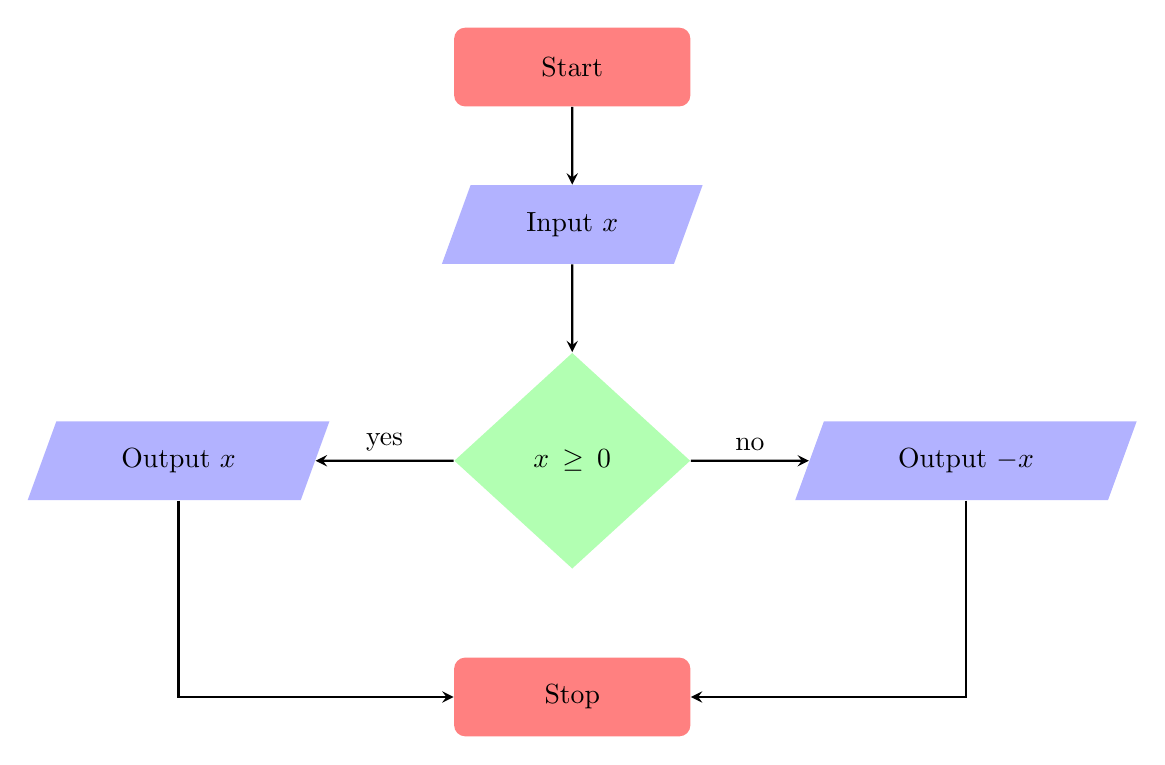
\begin{tikzpicture}
    \node [startstop] at (0,0) (start) {Start};
    \node [io] at (0,-2) (io1) {Input $x$};
    \node [decision] at (0,-5) (decision) {$x\geq 0$};
    \node [io] at (5,-5) (io2) {Output $-x$};
    \node [io] at (-5,-5) (io3) {Output $x$};
    \node [startstop] at (0,-8) (stop) {Stop};
    \draw [arrow] (start) -- (io1);
    \draw [arrow] (io1) -- (decision);
    \draw [arrow] (decision) -- node[anchor=south] {no}(io2);
    \draw [arrow] (decision) -- node[anchor=south] {yes} (io3);
    \draw [arrow] (io2) |- (stop);
    \draw [arrow] (io3) |- (stop);
    \end{tikzpicture}
\end{center}
\begin{center}
    Figure 1: An example of an algorithm that computes $|x|$.
\end{center}


In Python we can implement this short algorithm using the following syntax:

\begin{verbatim}
==============================
if condition:
        code1
else:
        code2
==============================
\end{verbatim}

The term \verb|condition| indicates the condition we wish to check. If the condition evaluates to \verb|True|, then the instructions given by \verb|code1| are followed. If the condition evaluates to \verb|False|, then the instructions given by \verb|code2| are followed. Using the template above, we can now write the necessary Python code to compute $|x|$.

\begin{verbatim}
==============================
if x > 0:
        absVal = x
else:
        absVal = -x
==============================
\end{verbatim}

The code above creates a variable \verb|absVal| that is assigned the absolute value of $x$ for any given $x$. The SageCell below shows how to use this code in practice. We assign the desired output to a variable so that we can use it later for whatever we want.

\begin{verbatim}
==============================
x = -3               # change this value and evaluate the cell to compute |x| for other x values

if x > 0:
        absVal = x
else:
        absVal = -x
print(absVal)        # this line prints the value of absVal to the screen to show that the variable has been assigned the correct value
==============================
\end{verbatim}

Note that in Python, whitespace (indentation) determines which lines of code belong to a particular code block. For example, the following code differs from that in the SageCell above in that the \verb|print| statement is only called if $x\leq 0$.

\begin{verbatim}
==============================
x = 4

if x > 0:
        absVal = x
else:
        absVal = -x
print(absVal)
==============================
\end{verbatim}

The example above shows how a flowchart with a decision compartment can be translated to Python code and vice versa. With enough practice one shoud be able to go between the two. Eventually, with enough experience, one can start coding without explicitly drawing a flowchart each time.

\section{Elif}

Below we give examples of how to expand on the basic if/else form to handle cases where multiple decisions are needed or if a decision has more than two outcomes.

The flowchart below (see Figure 2) shows an algorithm for computing the $sgn$ function seen in the Flowchart problem section.

\begin{center}
    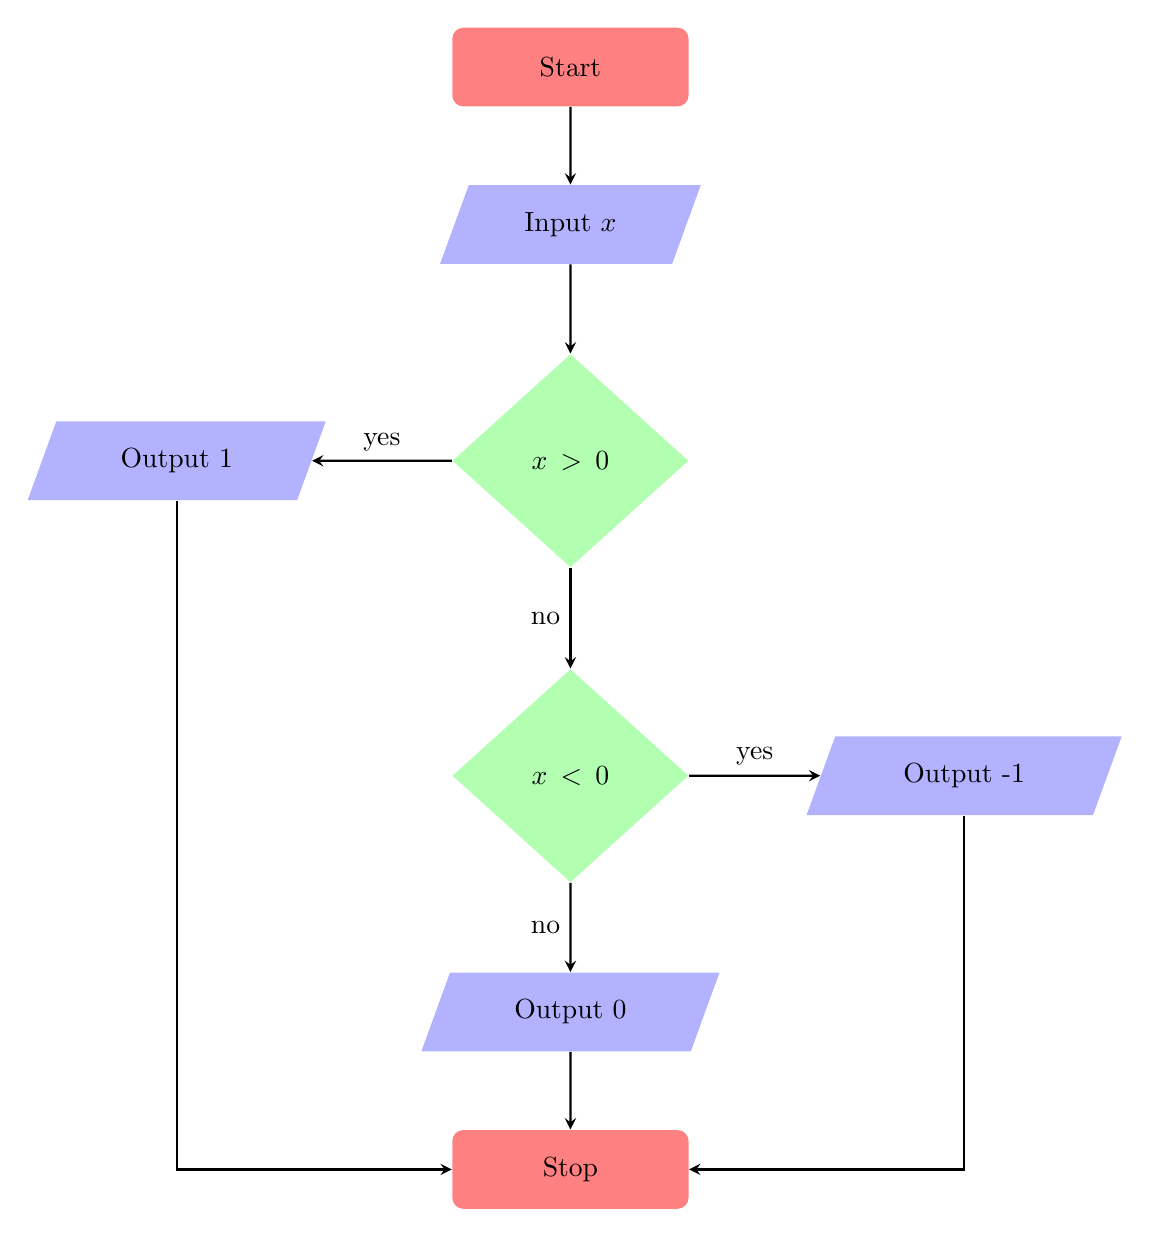
\begin{tikzpicture}
    \node [startstop] at (0,0) (start) {Start};
    \node [io] at (0,-2) (io1) {Input $x$};
    \node [decision] at (0,-5) (decision1) {$x>0$};
    \node [io] at (-5,-5) (io2) {Output 1};
    \node [decision] at (0,-9) (decision2) {$x<0$};
    \node [io] at (5,-9) (io3) {Output -1};
    \node [io] at (0,-12) (io4) {Output 0};
    \node [startstop] at (0,-14) (stop) {Stop};
    \draw [arrow] (start) -- (io1);
    \draw [arrow] (io1) -- (decision1);
    \draw [arrow] (decision1) -- node[anchor=south] {yes}(io2);
    \draw [arrow] (decision1) -- node[anchor=east] {no} (decision2);
    \draw [arrow] (decision2) -- node[anchor=south] {yes} (io3);
    \draw [arrow] (decision2) -- node[anchor=east] {no} (io4);
    \draw [arrow] (io2) |- (stop);
    \draw [arrow] (io3) |- (stop);
    \draw [arrow] (io4) -- (stop);
    \end{tikzpicture}
\end{center}
\begin{center}
    Figure 2: An algorithm that determines the sign of a real number $x$.
\end{center}

This can be implemented in Python in several ways.

We can put an if/else statement inside of another if or else block of code. Note the indentation of the lines belonging to the second if/else statement.

\begin{verbatim}
==============================
x = -5
if x > 0:
        sgn = 1
else:
        if x < 0:
                sgn = -1
        else:
                sgn = 0
print(sgn)
==============================
\end{verbatim}
	
We can use the \verb|elif| (else-if) option that simply shortens the code above.

\begin{verbatim}
===PSEUDOCODE================
if condition1:
        code1
elif condition2:
        code2
elif condition3:
        code3
    ...
elif conditionk:
        codek
else:
        code(k+1)
==============================
\end{verbatim}

The \verb|elif| lines above allow one to write a program that checks multiple conditions. The program will execute whatever instructions are associated with the first (and only the first) condition checked that is satisfied. If none of the conditions are satisfied, then the default behavior is given by the code in the \verb|else| portion.

\begin{verbatim}
==============================
x = 4
if x > 0:
        sgn = 1
elif x < 0:
        sgn = -1
else:
        sgn = 0
print(sgn)
==============================
\end{verbatim}

Note that the second option greatly increases the readability of the code and can be expanded with more \verb|elif| lines if more options must be considered.

Finally, a condition checked by an if/elif statement need not involve a comparison operator. Any nonzero number is treated as \verb|True|, while zero is treated as \verb|False|. See the example below.

\begin{verbatim}
==============================
x = 3
if x:
       print(1)
else:
       print(0)
==============================
\end{verbatim}

\section{Problems}

\begin{question}
Define the Heaviside step function $H$ for any real number $x$ as
	$$H(x)=\begin{cases} 1 &\text{ if $x\geq 0$}\\
		0 &\text{ otherwise.}
	\end{cases}$$
Develop an algorithm to implement the Heaviside function. Express your algorithm as a flowchart and in Python. In Python, assign the desired output to a variable \verb|H|.
	\begin{hint}
		This problem is similar to computing $|x|$. Note that the second hint for this problem is the solution.
	\end{hint}
	\begin{hint}
	\begin{center}
            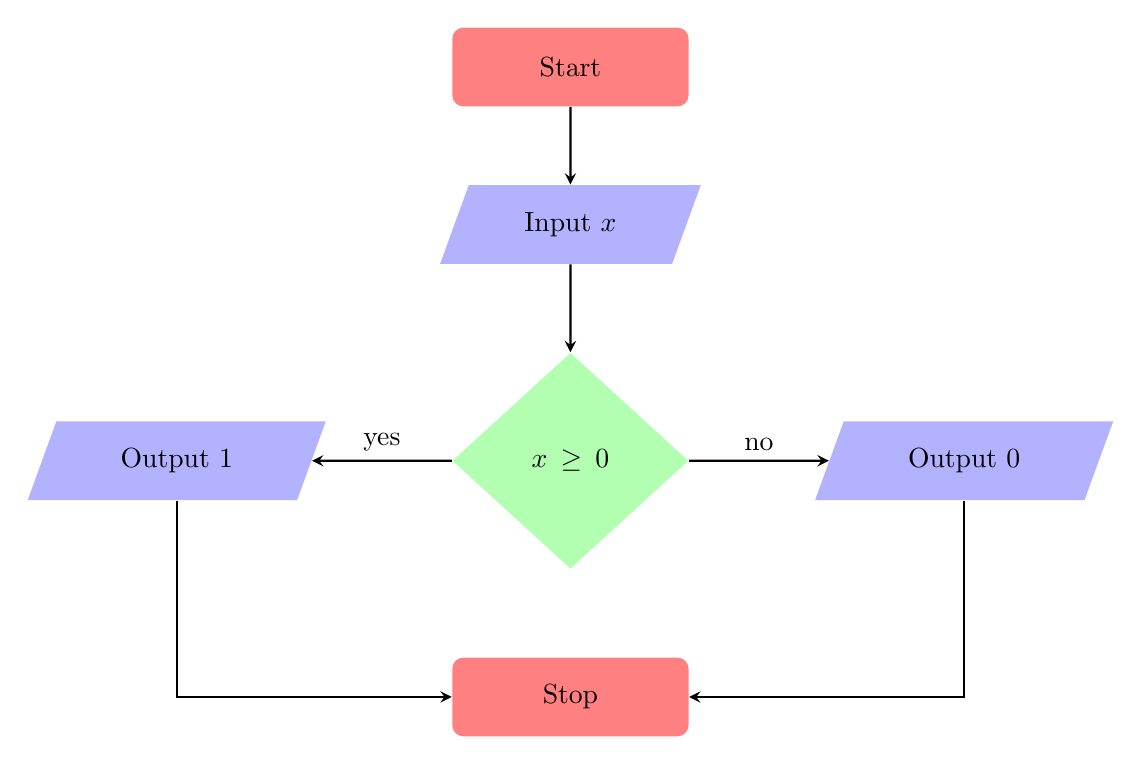
\begin{tikzpicture}
            \node [startstop] at (0,0) (start) {Start};
            \node [io] at (0,-2) (io1) {Input $x$};
            \node [decision] at (0,-5) (decision) {$x\geq 0$};
            \node [io] at (5,-5) (io2) {Output $0$};
            \node [io] at (-5,-5) (io3) {Output $1$};
            \node [startstop] at (0,-8) (stop) {Stop};
            \draw [arrow] (start) -- (io1);
            \draw [arrow] (io1) -- (decision);
            \draw [arrow] (decision) -- node[anchor=south] {no}(io2);
            \draw [arrow] (decision) -- node[anchor=south] {yes} (io3);
            \draw [arrow] (io2) |- (stop);
            \draw [arrow] (io3) |- (stop);
            \end{tikzpicture}
	\end{center}
\begin{verbatim}
==============================
if x >= 0:
        H = 1
else:
        H = 0
==============================
\end{verbatim}
	\end{hint}
\end{question}

\begin{question}
A different definition of the Heaviside step function gives a different value at $x=0$, namely,
	$$H(x)=\begin{cases} 1 &\text{ if $x>0$}\\
		1/2 &\text{ if $x=0$}\\
		0 &\text{ otherwise.}
	\end{cases}$$
Develop an algorithm to implement this alternative Heaviside function. Express your algorithm as a flowchart and in Python. In Python, assign the desired output to a variable \verb|H|.
	\begin{hint}
		This problem is similar to computing $sgn(x)$. Note that the second hint for this problem is the solution.
	\end{hint}
	\begin{hint}
	\begin{center}
            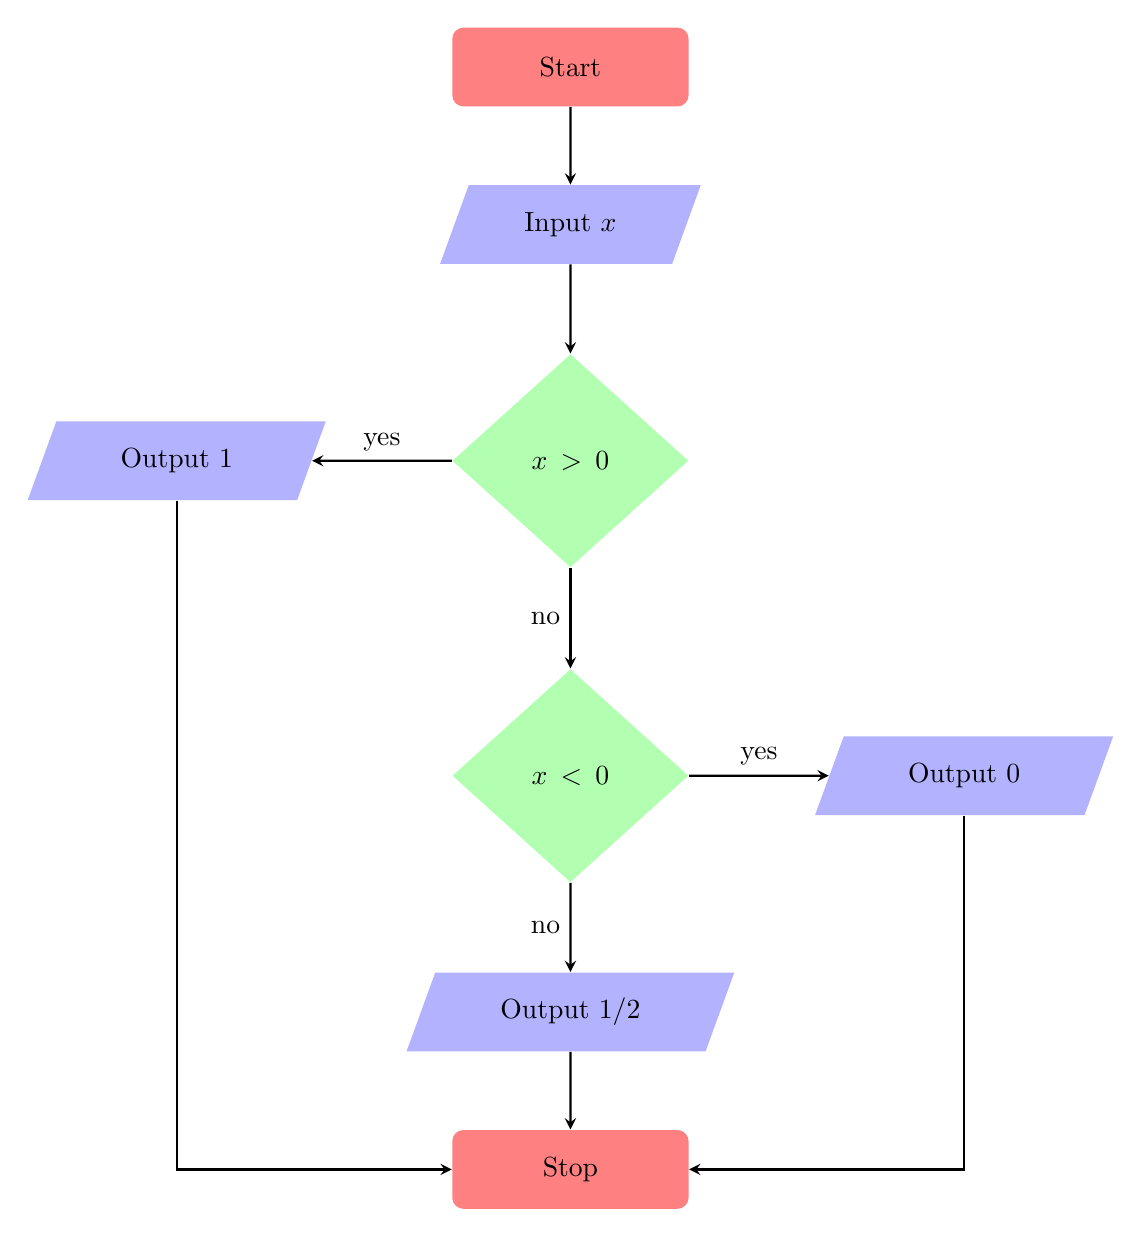
\begin{tikzpicture}
            \node [startstop] at (0,0) (start) {Start};
            \node [io] at (0,-2) (io1) {Input $x$};
            \node [decision] at (0,-5) (decision1) {$x>0$};
            \node [io] at (-5,-5) (io2) {Output 1};
            \node [decision] at (0,-9) (decision2) {$x<0$};
            \node [io] at (5,-9) (io3) {Output 0};
            \node [io] at (0,-12) (io4) {Output 1/2};
            \node [startstop] at (0,-14) (stop) {Stop};
            \draw [arrow] (start) -- (io1);
            \draw [arrow] (io1) -- (decision1);
            \draw [arrow] (decision1) -- node[anchor=south] {yes}(io2);
            \draw [arrow] (decision1) -- node[anchor=east] {no} (decision2);
            \draw [arrow] (decision2) -- node[anchor=south] {yes} (io3);
            \draw [arrow] (decision2) -- node[anchor=east] {no} (io4);
            \draw [arrow] (io2) |- (stop);
            \draw [arrow] (io3) |- (stop);
            \draw [arrow] (io4) -- (stop);
            \end{tikzpicture}
	\end{center}
\begin{verbatim}
==============================
if x > 0:
        H = 1
elif x == 0:
        H = 0.5
else:
        H = 0
==============================
\end{verbatim}
	\end{hint}
\end{question}

\begin{question}
	Express your algorithm solution from the first question in the Flowcharts with Operators section in Python. In Python, assign the desired output to a variable \verb|real_roots|.  Note that the hint for this problem is the solution.
	\begin{hint}
\begin{verbatim}
==============================
if b**2-4*a*c >= 0:
        real_roots = 1
else:
        real_roots = 0
==============================
\end{verbatim}
	\end{hint}
\end{question}

\begin{question}
	Develop an algorithm that takes in three real numbers $a$, $b$, and $c$ with $a\neq 0$ and determines the number of distict real roots of the quadratic polynomial $ax^2+bx+c$. The output should be the the number of distinct real roots. Express your algorithm as a flowchart and in Python. In Python, assign the desired output to a variable \verb|real_roots_count|.
	\begin{hint}
	As in the previous problem, the solution is dependent on the value of the quantity $b^2-4ac$. Note that the second hint for this problem is the solution.
	\end{hint}
	\begin{hint}
            \begin{center}
               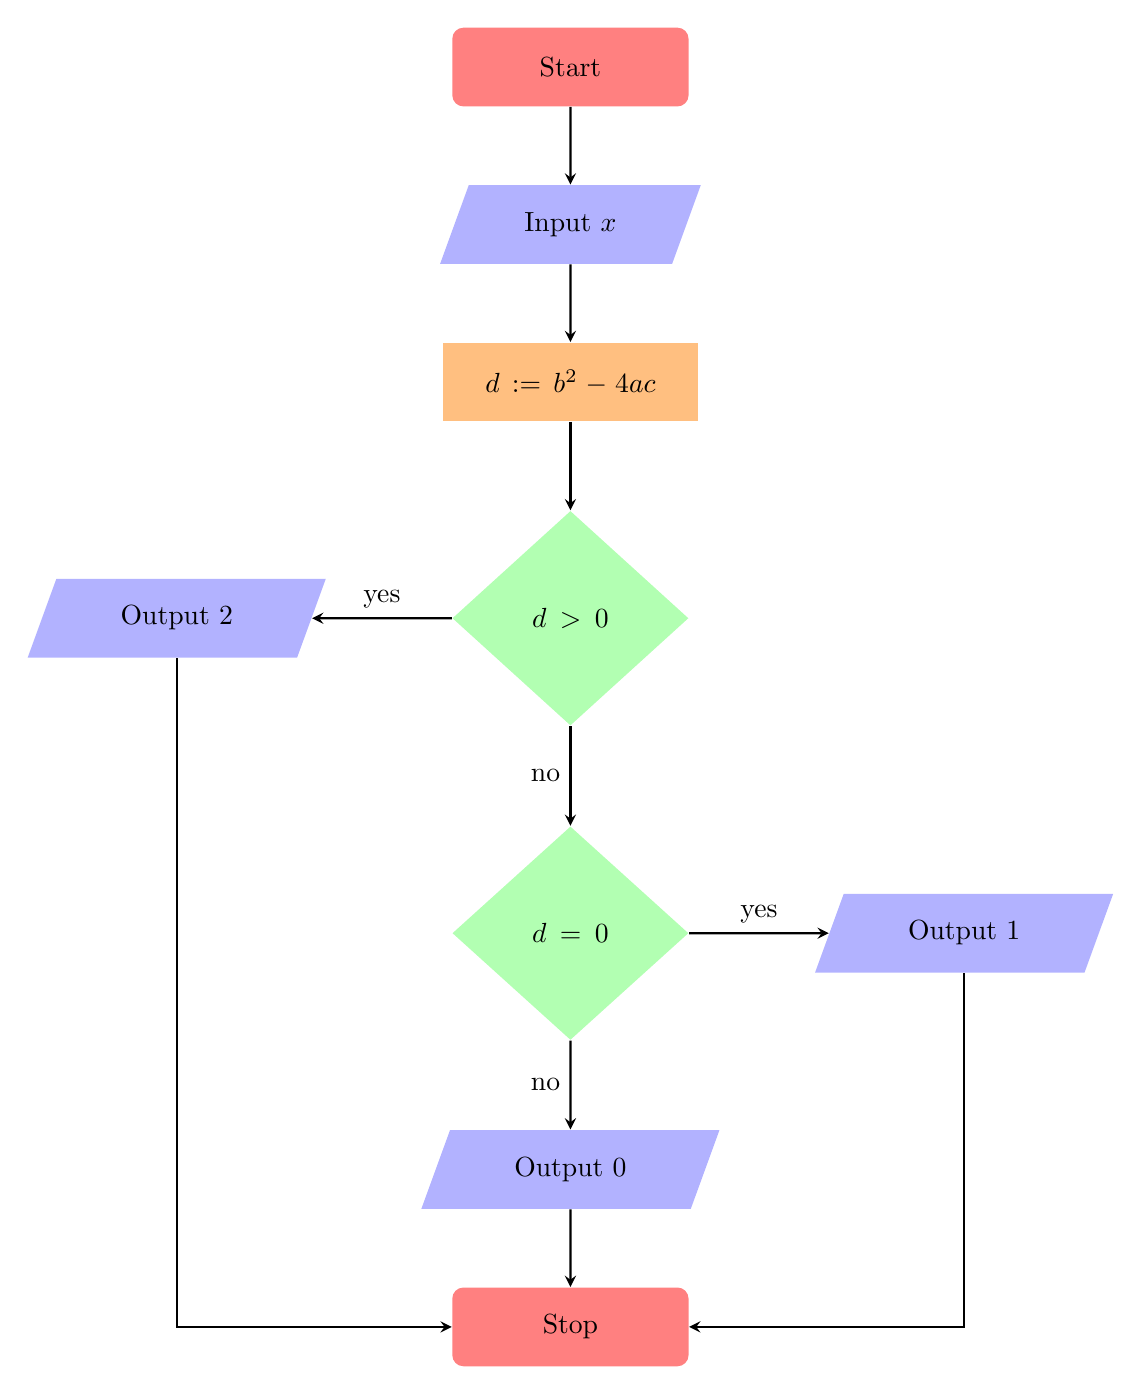
\begin{tikzpicture}
               \node [startstop] at (0,2) (start) {Start};
               \node [io] at (0,0) (io1) {Input $x$};
               \node [process] at (0,-2) (process) {$d:=b^2-4ac$};
               \node [decision] at (0,-5) (decision1) {$d>0$};
               \node [io] at (-5,-5) (io2) {Output 2};
               \node [decision] at (0,-9) (decision2) {$d=0$};
               \node [io] at (5,-9) (io3) {Output 1};
               \node [io] at (0,-12) (io4) {Output 0};
               \node [startstop] at (0,-14) (stop) {Stop};
               \draw [arrow] (start) -- (io1);
               \draw [arrow] (io1) -- (process);
               \draw [arrow] (process) -- (decision1);
               \draw [arrow] (decision1) -- node[anchor=south] {yes}(io2);
               \draw [arrow] (decision1) -- node[anchor=east] {no} (decision2);
               \draw [arrow] (decision2) -- node[anchor=south] {yes} (io3);
               \draw [arrow] (decision2) -- node[anchor=east] {no} (io4);
               \draw [arrow] (io2) |- (stop);
               \draw [arrow] (io3) |- (stop);
               \draw [arrow] (io4) -- (stop);
               \end{tikzpicture}
           \end{center}
\begin{verbatim}
==============================
if b**2-4*a*c > 0:
        real_roots_count = 2
elif b**2-4*a*c == 0:
        real_roots_count = 1
else:
        real_roots_count = 0
==============================
\end{verbatim}
	\end{hint}
\end{question}

\begin{question}
	Suppose you are given three distinct real numbers $A$, $B$, and $C$. Develop an algorithm that determines which one is the largest. Express your algorithm as a flowchart and in Python. In Python, assign the desired output to the variable \verb|maximum|. Note that the hint for this problem is the solution.
	\begin{hint}
	    \begin{center}
                 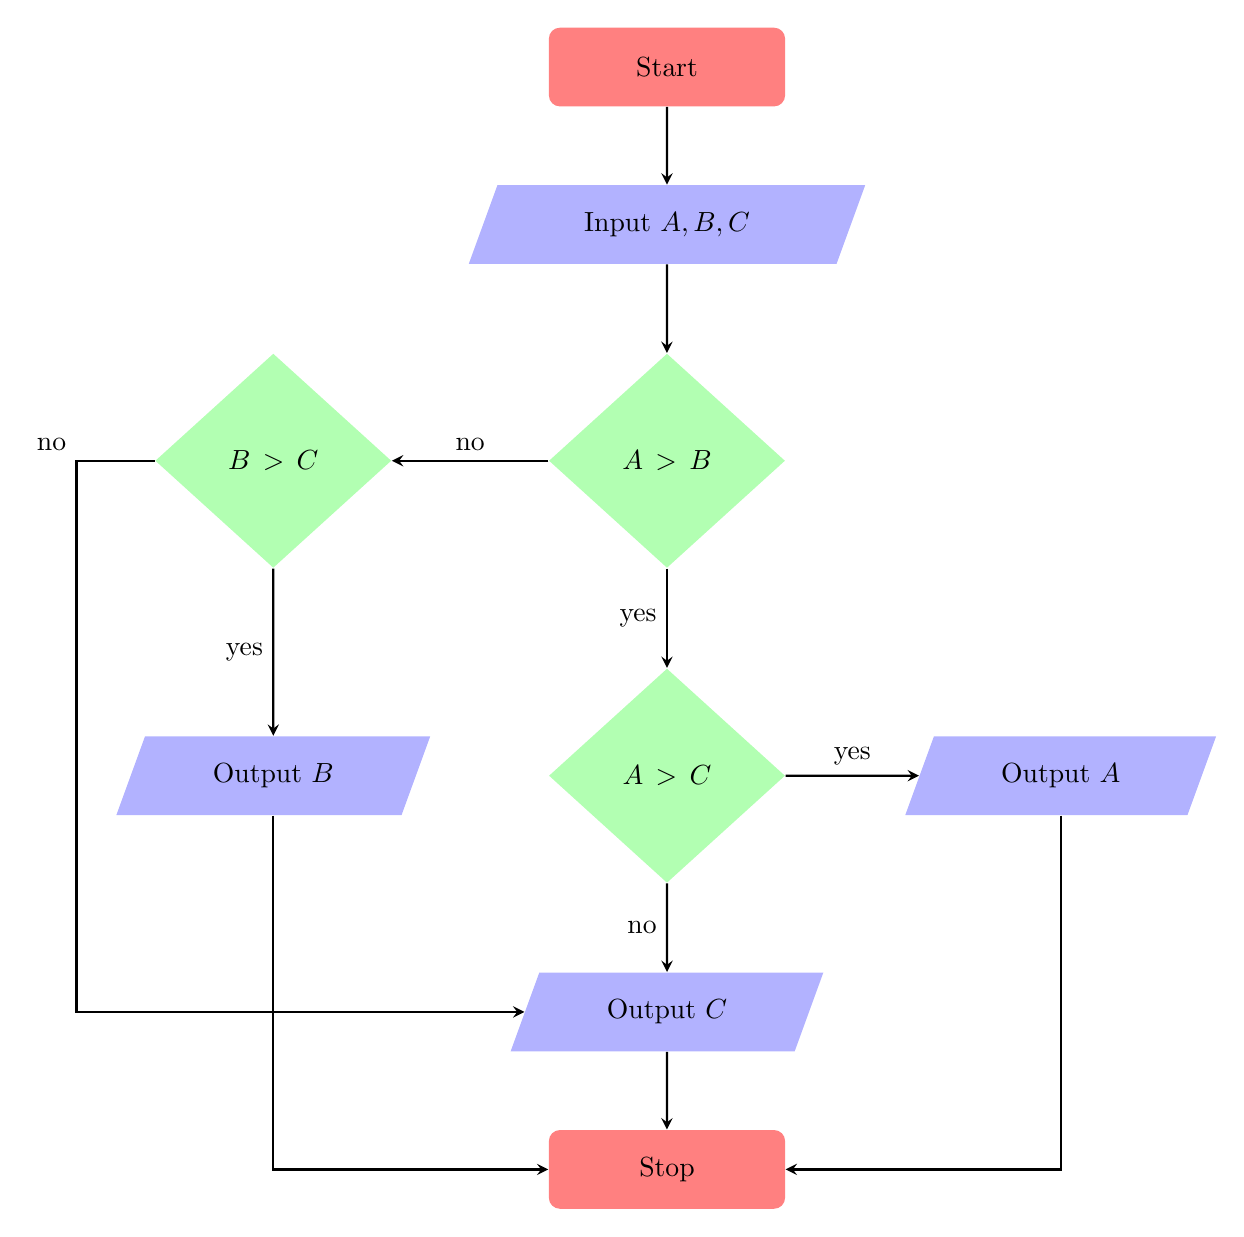
\begin{tikzpicture}
                 \node [startstop] at (0,0) (start) {Start};
                 \node [io] at (0,-2) (io1) {Input $A,B,C$};
                 \node [decision] at (0,-5) (decision1) {$A>B$};
                 \node [decision] at (-5,-5) (decision2) {$B>C$};
                 \node [decision] at (0,-9) (decision3) {$A>C$};
                 \node [io] at (-5,-9) (io2) {Output $B$};
                 \node [io] at (5,-9) (io3) {Output $A$};
                 \node [io] at (0,-12) (io4) {Output $C$};
                 \node [startstop] at (0,-14) (stop) {Stop};
                 \draw [arrow] (start) -- (io1);
                 \draw [arrow] (io1) -- (decision1);
                 \draw [arrow] (decision1) -- node[anchor=south] {no} (decision2);
                 \draw [arrow] (decision2) -- node[anchor=east] {yes} (io2);
                 \draw [arrow] (decision1) -- node[anchor=east] {yes} (decision3);
                 \draw [arrow] (decision3) -- node[anchor=south] {yes} (io3);
                 \draw [arrow] (decision3) -- node[anchor=east] {no} (io4);
                 \draw [arrow] (decision2) -| node[anchor=south east] {no} (-7.5,-5) |-  (io4);
                 \draw [arrow] (io2) |- (stop);
                 \draw [arrow] (io3) |- (stop);
                 \draw [arrow] (io4) -- (stop);
                 \end{tikzpicture}
            \end{center}
\begin{verbatim}
==============================
if A > B:
        if A > C:
                maximum = A
        else:
                maximum = C
else:
        if B > C:
                maximum = B
        else:
                maximum = C
==============================
\end{verbatim}
	\end{hint}
\end{question}

\end{document}
